\section{UML export}

In this section we will show you how you can create and view \emph{UML} diagrams from a \emph{Reprotool} project. Although it is not
absolutely neccesary, it is preferrable that you install now into reprotool the \emph{UML2 Tools} eclipse plugin.

\subsection{Installing \emph{UML2 Tools} into \emph{Reprotool}}

Download the following zip archive \url{http://download.eclipse.org/modeling/mdt/uml2tools/downloads/drops/0.10.0/I201103290512/mdt-uml2tools-Update-incubation-I201103290512.zip}
on your filesystem. Now execute the command
\begin{verbatim}
 Help / Install New Software...
\end{verbatim}
Now click on the \emph{Add} button. A small dialog box appears now. Here click the \emph{Archive} button and select the zip archive
you just downloaded. Click OK. Now you are back to the \emph{Install} dialog. Here select the \emph{UML2 Tools (Incubation)} item and
click next. Now simply proceed with the installation. After the successful installation, you will be asked to restart \emph{Eclipse}.
Now that's it, you have successfully installed the \emph{UML2 Tools} eclipse package.

\subsection{UML Use-Case diagram}

Right-click on the \emph{Reprotool} project file in the \emph{Project explorer} and select the \emph{Conwert SW project to UML use case
diagram} command. After that you should note a new file in the \emph{Project explorer} with the \emph{.swproj.uc.uml} file extension.
Right-click this file and select the \emph{Initialize Use Case Diagram} command. Now just click \emph{Finish}. An UML diagram should
fire up in a new editor instance. In the next figure you can see a use-case diagram of the \emph{IncludeDemo} example project.

\newpage

\begin{figure}[ht]
  \centering
  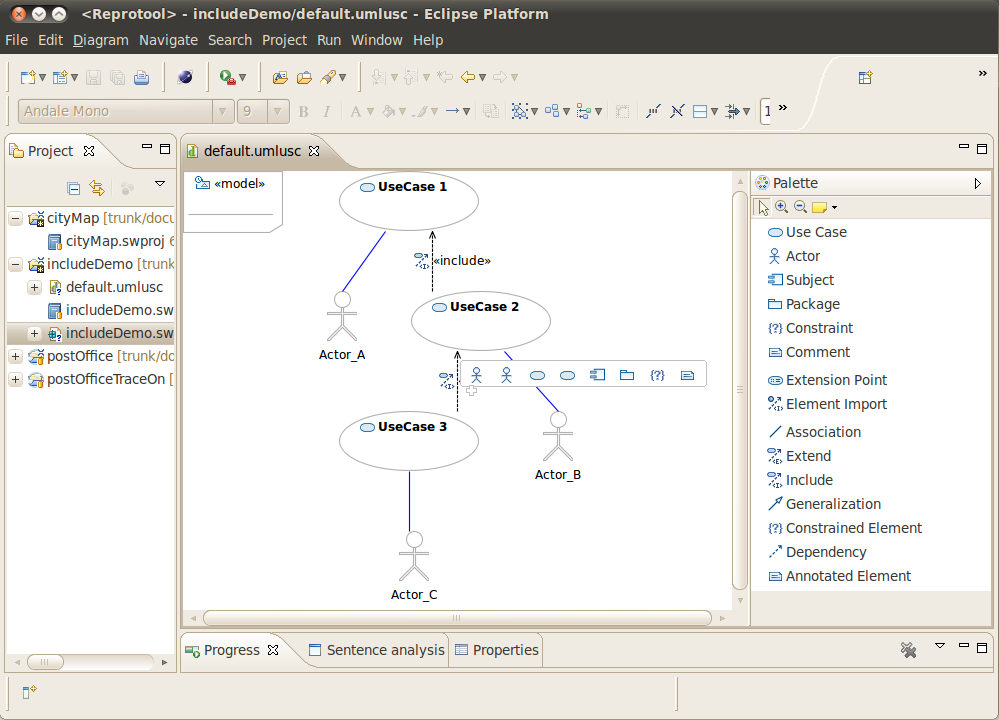
\includegraphics[height=280pt]{images/reprotoolUCDiagram}
  \caption{Use-case diagram of the \emph{IncludeDemo Reprotool} example project}
  \label{fig:reprotoolUCDiagram}
\end{figure}

\subsection{UML Class diagram}

Right-click on the \emph{Reprotool} project file in the \emph{Project explorer} and select the \emph{Conwert SW project to UML class
diagram} command. After that you should note a new file in the \emph{Project explorer} with the \emph{.swproj.class.uml} file extension.
Right-click this file and select the \emph{Initialize Class Diagram} command. Now just click \emph{Finish}. An UML class diagram should
fire up in a new editor instance.